\documentclass[12pt]{amsart}

\addtolength{\hoffset}{-2.25cm}
\addtolength{\textwidth}{4.5cm}
\addtolength{\voffset}{-2.5cm}
\addtolength{\textheight}{5cm}
\setlength{\parskip}{0pt}
\setlength{\parindent}{15pt}

\usepackage{amsthm}
\usepackage{amsmath}
\usepackage{amssymb}
\usepackage[colorlinks = true, linkcolor = black, citecolor = black, final]{hyperref}

\usepackage{graphicx}
\usepackage{multicol}
\usepackage{ marvosym }
\usepackage{wasysym}
\usepackage{tikz}
\usetikzlibrary{patterns}

\newcommand{\ds}{\displaystyle}
\DeclareMathOperator{\sech}{sech}


\setlength{\parindent}{0in}

\pagestyle{empty}

\begin{document}

\thispagestyle{empty}

{\scshape Math 2400} \hfill {\scshape \large Project \#3 - Center of Mass} \hfill {\scshape Spring 2016}
 
\smallskip

\hrule

\bigskip

We need some more Math Department decorations, so we're going to build a mobile that demonstrates our mastery of the concept of the center of mass of an two dimensional object.  Yay!  This is going to be a collective big group effort, since we will have a single final product, but everyone will contribute a shape to hang from the mobile and submit an individual write-up.

\bigskip

\bigskip

The basic process will be:

\begin{enumerate}

\item  Design and build a cool shape.

\medskip

\item  Surround that shape with card-stock and/or pretty paper to keep it all together.

\medskip

\item  Find the center of mass of that object.

\medskip

\item  Test it and make sure it is reasonable.

\medskip

\item  Clearly mark the coordinates on the object itself as well as the total mass.

\medskip

\item  Attach a string to the object at the center of mass so that it will hang from the string level with the floor.

\medskip

\item  Hang your object from the mobile in a way that keeps the entire mobile balanced.

\medskip

\end{enumerate}

\bigskip

\bigskip

The only current rule (I may come up with more) is:

\begin{quote}The density of your final object should not be uniform.  So, use multiple plastic or felt shapes and/or add an extra shape to the card-stock cover. \end{quote}

\bigskip

\bigskip

The write-up you submit on Blackboard should include 
\begin{itemize}
\item  A diagram of the complete shape and all the specifications,
\item  The steps to compute the center of mass,
\item  An explanation of the computation and derivation of any new formulas, and
\item  A summary of any collaboration and computations needed to hang the final object and keep the whole system balanced.
\end{itemize}

\newpage

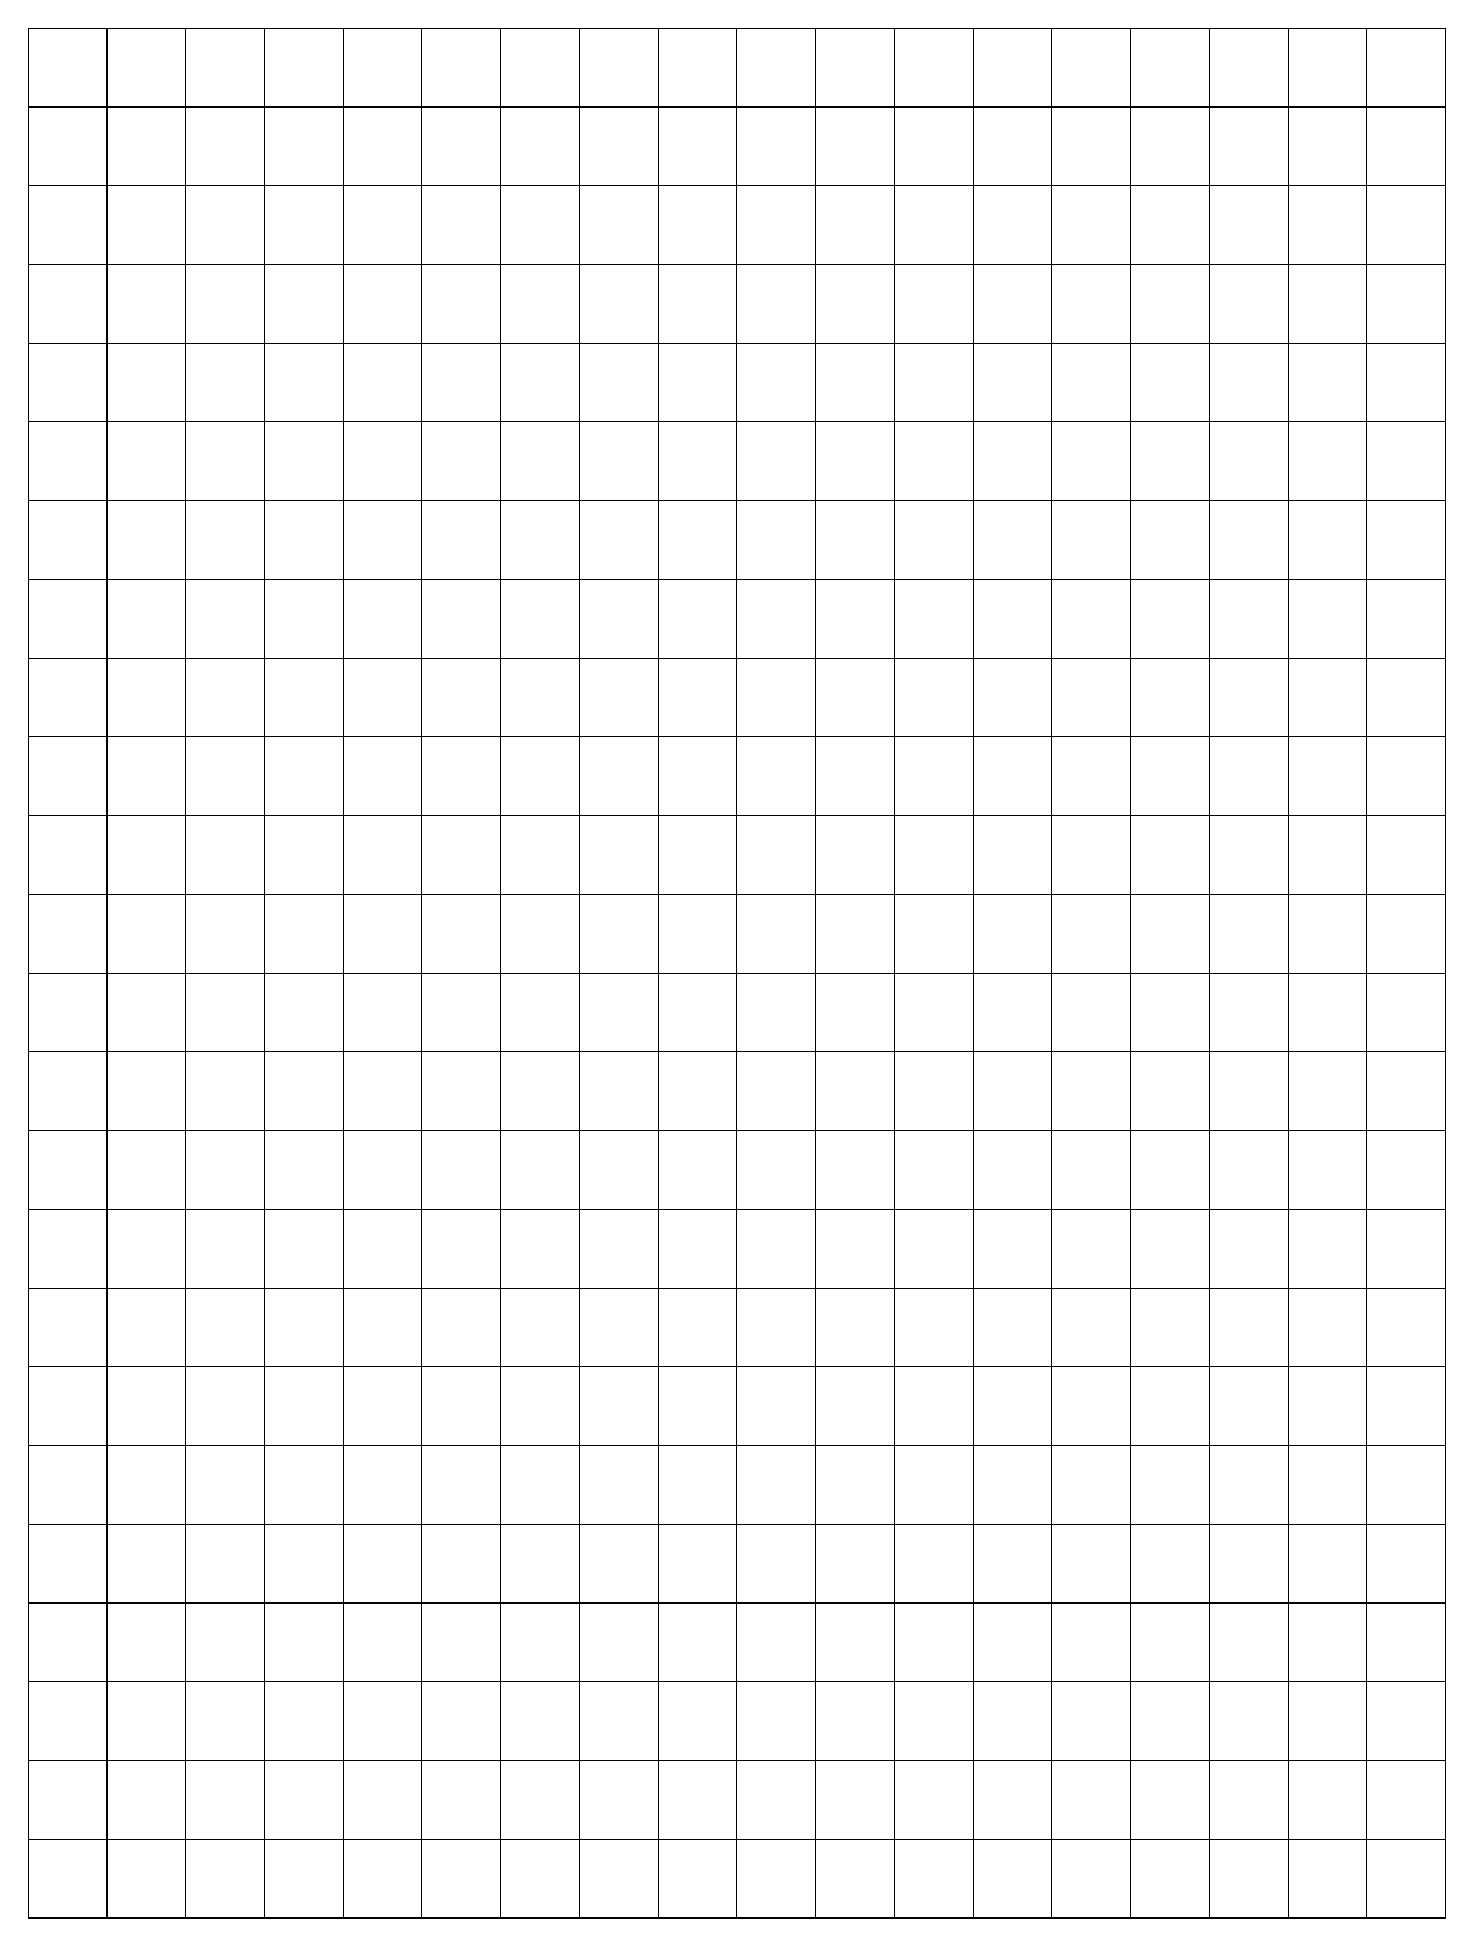
\begin{tikzpicture}
\draw (-6,-12) grid (12, 12);
\end{tikzpicture}

\newpage

{\bf The Shape:}  For my shape I chose a plastic square and a third of a circular disk.  I extended the card stock outer layer to include the triangle on the left side of the diagram above.  I measured the side of the square as well as the radius of the circle to be approximately 10cm.  After a bit of thinking, I chose to put the the origin at the lower left corner of the square to be the origin of the coordinate plane.

\bigskip

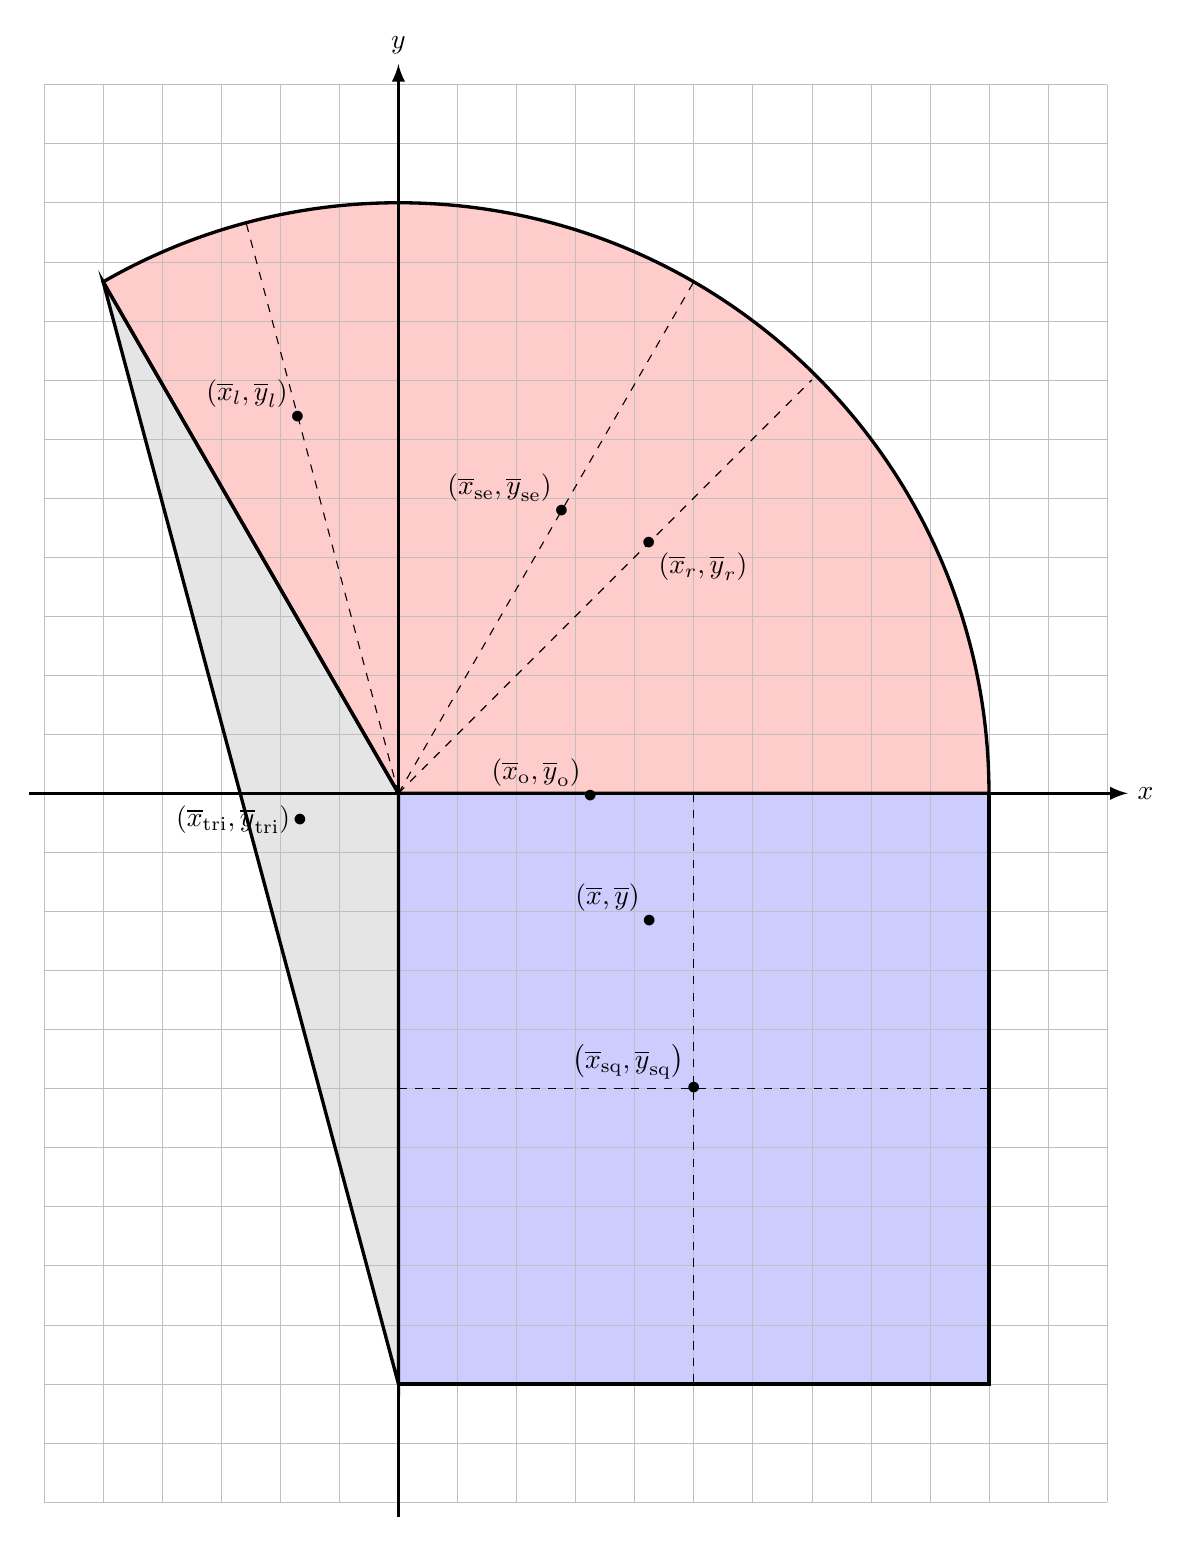
\begin{tikzpicture}[scale = .75]
\draw[fill = blue!20] (0,0) -- (10,0) -- (10,-10) -- (0, -10) -- cycle;
\draw[fill = red!20] (10,0) arc (0:120:10) -- (0,0) -- cycle;
\draw[fill = gray!20] (-5,8.66)--(0,0)--(0,-10)--cycle;
\draw[very thin, gray!50] (-6,-12) grid (12, 12);
\draw[very thick] (0,0) --(10,0) -- (10,-10) -- (0, -10) -- cycle;
\draw[very thick] (10,0) arc (0:120:10) -- (0,0) -- cycle;
\draw[very thick] (-5,8.66)--(0,0)--(0,-10)--cycle;
\node at (-1.6666666, -.45) {$\bullet$};
\node[anchor = east] at (-1.6666666, -.45) {$\left(\overline{x}_{\text{tri}}, \overline{y}_{\text{tri}}\right)$};
\node at (5, -5) {$\bullet$};
\node[anchor = south east] at (5, -5) {$\left(\overline{x}_{\text{sq}},\overline{y}_{\text{sq}}\right)$};
\node at (2.76, 4.77) {$\bullet$};
\node[anchor = south east] at (2.76, 4.77) {$\left(\overline{x}_{\text{se}},\overline{y}_{\text{se}}\right)$};
\node at (3.25, -.05) {$\bullet$};
\node[anchor = south east] at (3.25, -.05) {$\left(\overline{x}_{\text{o}},\overline{y}_{\text{o}}\right)$};
\node at (4.25, -2.16) {$\bullet$};
\node[anchor = south east] at (4.25, -2.16) {$\left(\overline{x},\overline{y}\right)$};

\node at (4.24, 4.24) {$\bullet$};
\node[anchor = north west] at (4.24, 4.24) {$(\overline{x}_r, \overline{y}_r)$};

\node at (-1.71, 6.37) {$\bullet$};
\node[anchor = south east] at (-1.71, 6.37) {$(\overline{x}_l, \overline{y}_l)$};

\draw[very thick, -latex] (-6.25, 0) -- (12.35, 0);
\node[anchor = west] at (12.35, 0) {$x$};

\draw[very thick, -latex] (0, -12.25) -- (0, 12.35);
\node[anchor = south] at (0, 12.35) {$y$};

\draw[dashed] (5, 0) -- (5, -10);
\draw[dashed] (0, -5) -- (10, -5);

\draw[dashed] (0,0) -- (5, 8.66);

\draw[dashed] (0,0) -- (7,7);

\draw[dashed] (0,0) -- (-2.59, 9.7);
\end{tikzpicture}

\bigskip

The points and dotted lines are various centers of mass and lines of symmetry that will be discussed further as we compute things.

\newpage

{\bf The Masses:} The mass of the entire square is 28 g and the circular sector has a mass of 9 g.  To compute the mass of the card-stock outer layers, I used the scale to determine the mass of a complete file folder, which was 22 grams, and measured the dimensions of the folder to get the area of 1323 cm$^2$.  I computed the area of my entire shape:
\begin{align*}A & = A_{\text{sq}} + A_{\text{se}} + A_{\text{tri}}\\
& = s^2 + \frac{1}{3}\pi r^2 + \frac{1}{2}bh\\
& = (10)(10) + \frac{1}{3}\pi(10)^2 + \frac{1}{2}(10)(5)\\
& = 100 + \frac{100\pi}{3} + 25\\
& = \frac{375 + 100\pi}{3}\\
& \approx 230\text{ cm}^2.
\end{align*}
My finished shape is made of two of these pieces of exactly the same dimensions, so the total area of card stock that I have is about 460 cm$^2$. Since the total amount of card stock was 1323 cm$^2$, and I used 460 cm$^2$, the mass for both pieces is
$$m = \frac{22\text{ g}}{1323\text{ cm}^2}\big(460\text{ cm}^2\big) \approx 8\text{ g}.$$

Since each shape has uniform density on its own, we can temporarily ignore the masses of each shape while we determine their respective centers of mass.

\bigskip

{\bf The Individual Centers of Mass:} Since the square has a bunch of symmetries, it is the easiest to find its center of mass; it is the center of the square!  With this assignment of the coordinate axes, that means the center of mass of the square is at $$\left(\overline{x}_{\text{sq}}, \overline{y}_{\text{sq}}\right) = (5,-5).$$
The center of mass of of the triangle part requires a bit more computational work, but we can use the fact we discovered in \#4 and \#5 of the Center of Mass worksheet; the center of mass of a triangle of uniform density is the same as the center of mass of the system of three equal point masses at the vertices.
\begin{align*}
(\overline{x}_{\text{tri}}, \overline{y}_{\text{tri}}) &  = \left(\frac{v_{1x} + v_{2x} + v_{3x}}{3}, \frac{v_{1y} + v_{2y} + v_{3y}}{3} \right)\\
& =\left(\frac{-5 + 0 + 0}{3},\frac{5\sqrt{3} + 0 + (-10)}{3} \right)\\
& = \left(-\frac{5}{3}, \frac{5\sqrt{3} - 10}{3}\right).
\end{align*}
The center of mass of the last piece, the circular sector, is the most difficult. There is likely a clever symmetry argument to be made, but we can also just use the formulas developed in class.  We'll need two separate integral calculations, since the lower boundary is given by two different lines, the $x$-axis for the right portion and the function $y = -\sqrt{3}x$ for the left portion.  The right portion is easier; because of symmetry the center of mass should lie on the line $y = x$, so we need only fine one coordinate.  The two integrals we would need to compute are $$\int_0^{10} \frac{1}{2}\left(\left(\sqrt{100 - x^2}\right)^2 - (0)^2\right)\,dx \hspace{.2in} \text{ and } \hspace{.2in} \int_0^{10} x\left(\sqrt{100 - x^2} - 0\right)\,dx.$$
The second of these integrals requires substitution, so we'll evaluate the first:
\begin{align*}
\int_0^{10} \frac{1}{2}\left(\left(\sqrt{100 - x^2}\right)^2 - (0)^2\right)\,dx & = \frac{1}{2}\int_0^{10} 100 - x^2\,dx\\
& = \frac{1}{2}\left[100x - \frac{x^3}{3}\right]_0^{10}\\
& = \frac{1}{2}\left[\left(100(10) - \frac{1000}{3}\right) - \left(0\right)\right]\\
& = \frac{1000}{3}.
\end{align*}
This is the numerator of the $x$-coordinate of the center of mass, and the denominator is simply the area of this portion of the shape, $\frac{1}{4}\pi r^2 = 25\pi$.  So the coordinates of the center of mass of the right portion of the sector are $$\left(\overline{x}_r, \overline{y}_r\right) = \left(\frac{1000/3}{25\pi}, \frac{1000/3}{25\pi}\right) = \left(\frac{40}{3\pi}, \frac{40}{3\pi}\right).$$
Now for the left portion. The denominator in each computation will be the area of the shape, $\frac{1}{12}\pi r^2 = \frac{25\pi}{3}$.  We'll multiply each of the necessary integrals by the reciprocal of this.
\begin{multicols}{2}
\hspace{-.25in}\begin{align*}
\overline{x}_l & = \frac{3}{25\pi}\int_{-5}^0 x\left(\sqrt{100 - x^2} - \left(-\sqrt{3}x\right)\right)\,dx \hspace{.25in}\\
& = \frac{3}{25\pi}\int_{-5}^0x\sqrt{100-x^2}\,dx + \frac{3\sqrt{3}}{25\pi}\int_{-5}^0 x^2\,dx\\
u & = 100 - x^2 \hspace{.3in} du = -2x\,dx\\
x & = 0 \rightarrow u = 100\\
x & = -5 \rightarrow u = 75\\
& = \frac{3}{25\pi}\int_{75}^{100} x\sqrt{u}\frac{du}{-2x} + \frac{3\sqrt{3}}{25\pi}\left[\frac{x^3}{3}\right]_{-5}^0\\
& = -\frac{3}{50\pi}\left[\frac{u^{3/2}}{3/2}\right]_{75}^{100} + \frac{\sqrt{3}}{25\pi}\left[0^3 - (-5)^3\right]\\
& = -\frac{1}{25\pi}\left[100^{3/2} - 75^{3/2}\right] + \frac{5\sqrt{3}}{\pi}\\
& = -\frac{1}{25\pi}\left[1000 - 375\sqrt{3}\right] + \frac{5\sqrt{3}}{\pi}\\
& = \frac{375\sqrt{3} - 1000 + 125\sqrt{3}}{25\pi}\\
& = \frac{20}{\pi}\left(\sqrt{3} - 2\right)
\end{align*}

\columnbreak

\begin{align*}
\hspace{.25in}\overline{y}_l& = \frac{3}{25\pi}\int_{-5}^0 \frac{1}{2}\left(\left(\sqrt{100 - x^2}\right)^2 - \left(-\sqrt{3}x\right)^2\right)\,dx\\
& = \frac{3}{50\pi}\int_{-5}^0 100 - x^2 - 3x^2\,dx\\
& = \frac{3}{50\pi}\int_{-5}^0 100 - 4x^2\,dx\\
& = \frac{3}{50\pi}\left[100x - \frac{4}{3}x^3\right]_{-5}^0\\
& = \frac{3}{50\pi}\left[(0) - \left(100(-5) - \frac{4}{3}(-5)^3\right)\right]\\
& = -\frac{3}{50\pi}\left(-500 + \frac{4(125)}{3}\right)\\
& = \frac{20}{\pi}
\end{align*}

\end{multicols}

Now that we have the center of mass for each portion of the sector, we can treat those portions as point masses and find the center of mass of the system of two points.
\begin{align*} \left( \overline{x}_{\text{se}}, \overline{y}_{\text{se}}\right) & = \left(\frac{\overline{x}_rm_r + \overline{x}_lm_l}{m_r + m_l}, \frac{\overline{y}_rm_r + \overline{y}_lm_l}{m_r + m_l} \right)\\ 
& = \left(\frac{25\pi\left( \frac{40}{3\pi}\right) + \frac{25\pi}{3}\left(\frac{20}{\pi}\left(\sqrt{3} - 2\right)\right)}{25\pi + \frac{25\pi}{3}}, \frac{25\pi\left(\frac{40}{3\pi}\right) + \frac{25\pi}{3}\left(\frac{20}{\pi}\right)}{25\pi + \frac{25\pi}{3}} \right)\\
& = \left(\frac{\frac{1000}{3} + \frac{500\sqrt{3}}{3} - \frac{1000}{3}}{\frac{100\pi}{3}}, \frac{\frac{1000}{3} + \frac{500}{3}}{\frac{100\pi}{3}} \right)\\
& = \left(\frac{5\sqrt{3}}{\pi}, \frac{15}{\pi} \right)
\end{align*}
As a sanity check of sorts, if we take the $x$-coordinate and multiply by $\sqrt{3}$, we get the $y$-coordinate. That means this center of mass lies on the line $y = \sqrt{3}x$, which is exactly what we want since that is a line of symmetry of the sector.\\

Now that we have the center of mass of the square, triangle, and sector, we can treat each of those as point masses in order to find the center of mass of the outer layers of card stock. Since the card stock has uniform mass density, we compute this weighted average using area.
\begin{align*}\left(\overline{x}_o, \overline{y}_o\right) & = \left(\frac{\overline{x}_{\text{sq}}A_{\text{sq}} + \overline{x}_{\text{tri}}A_{\text{tri}} + \overline{x}_{\text{se}}A_{\text{se}}}{A_{\text{sq}} + A_{\text{tri}} + A_{\text{se}}} , \frac{\overline{y}_{\text{sq}}A_{\text{sq}} + \overline{y}_{\text{tri}}A_{\text{tri}} + \overline{y}_{\text{se}}A_{\text{se}}}{A_{\text{sq}} + A_{\text{tri}} + A_{\text{se}}}\right)\\
& = \left(\frac{(5)(100) + \left(-\frac{5}{3}\right)(25) + \left(\frac{5\sqrt{3}}{\pi}\right)\left(\frac{100\pi}{3}\right)}{100 + 25 + \frac{100\pi}{3}}, \frac{(-5)(100) + \left(\frac{5\sqrt{3} - 10}{3}\right)\left(25\right)+ \left(\frac{15}{\pi}\right)\left(\frac{100\pi}{3}\right)}{100 + 25 + \frac{100\pi}{3}} \right)\\
& = \left(\frac{500 - \frac{125}{3} + \frac{500\sqrt{3}}{3}}{125 + \frac{100\pi}{3}}, \frac{-500 + \frac{125\sqrt{3}}{3} - \frac{250}{3} + 500}{125 + \frac{100\pi}{3}} \right)\\
& = \left(\frac{1500 - 125 + 500\sqrt{3}}{375 + 100\pi}, \frac{-1500 + 125\sqrt{3} - 250 + 1500}{375 + 100\pi}\right)\\
& = \left(\frac{1375 + 500\sqrt{3}}{375 + 100\pi},\frac{125\sqrt{3} - 250}{375 + 100\pi} \right)\\
& = \left(\frac{55 + 20\sqrt{3}}{15 + 4\pi},\frac{5\sqrt{3} - 10}{15 + 4\pi} \right)
\end{align*}

All together for the center of mass of the entire shape:

\begin{align*}
\left(\overline{x}, \overline{y} \right) & = \left( \frac{\overline{x}_{\text{sq}}m_{\text{sq}} + \overline{x}_{\text{se}}m_{\text{se}} + \overline{x}_{\text{o}}m_{\text{o}}}{m_{\text{sq}} + m_{\text{se}} + m_{\text{o}}}, \frac{\overline{y}_{\text{sq}}m_{\text{sq}} + \overline{y}_{\text{se}}m_{\text{se}} + \overline{y}_{\text{o}}m_{\text{o}}}{m_{\text{sq}} + m_{\text{se}} + m_{\text{o}}}\right)\\
& = \left( \frac{(5)(28) + \left(\frac{5\sqrt{3}}{\pi}\right)(9) + \left(\frac{55 + 20\sqrt{3}}{15 + 4\pi}\right)(8)}{28 + 9 + 8}, \frac{(-5)(28) + \left(\frac{15}{\pi}\right)(9) + \left(\frac{5\sqrt{3} - 10}{15 + 4\pi}\right)(8)}{28 + 9 + 8}\right)\\
& = \left(\frac{140 + \frac{45\sqrt{3}}{\pi} + \frac{440 + 160\sqrt{3}}{15 + 4\pi}}{45}, \frac{-140 + \frac{135}{\pi} + \frac{40\sqrt{3} - 80}{15 + 4\pi}}{45}\right)\\
& \approx \left(4.25 , -2.16\right)
\end{align*}



All of the different centers of mass are marked on the diagram, and visually they make sense.  The shape is flat when hung from the center of mass, so that is also a good sign.

I have not hung up my shape yet as part of the mobile.  Since there is already a shape at the center of the mobile, I'll need a friend or two and their shapes to keep it balanced.  

Since we will all know the total masses of our shapes, we can set up the following equation:
$$\left(\frac{x_1m_1 + x_2m_2 + x_3m_3}{m_1 + m_2 + m_3}, \frac{y_1m_1 + y_2m_2 + y_3m_3}{m_1 + m_2 + m_3} \right) = (0,0)$$
where $(x_i, y_i)$ will be the coordinates where we hang our shapes, and $m_i$ are the masses of each shape.  The expression on the left represents the center of mass of the system of our three shapes, and we want that to be the center of the mobile, so we set it equal to $(0,0)$.  This is a system of two equations (one for each of the $x$ and $y$-coordinates) with three unknowns in each.  That means there will be multiple solutions.  I would propose starting by determining two possible points roughly at the vertices of an equilateral-ish triangle centered at the origin, then solving the equations for the third point.  Hopefully starting with those two points does not make either equation have no solution, but if it does, we can adjust!


\end{document}